\documentclass[12pt, a4paper]{report}
\usepackage[italian]{babel}
\usepackage[utf8]{inputenc}
\usepackage{amsmath, amsfonts, amssymb, amsthm}
\usepackage{graphicx}

\author{Athos Innocenti}
\title{\Huge Elettronica}\date{}\author{}
\begin{document}
\maketitle
\tableofcontents
\chapter{Semiconduttori}
I \textbf{semiconduttori} sono materiali parzialmente conduttori cioè hanno una conducibilità più alta degli \textit{isolanti} (materiali \textit{dielettrici} in cui gli elettroni sono fissi in un reticolo quindi sono incapaci di muoversi e per questo non scorre corrente), ma minore dei \textit{conduttori} (tutti i \textit{metalli} nei quali, se si applica un potenziale, scorre corrente perché ci sono elettroni liberi disponibili all'interno del materiale). Tendenzialmente i semiconduttori sono degli isolanti, ma sotto opportune condizioni si comportano come conduttori. In questi materiali gli atomi sono legati tra loro tramite legami \textbf{covalenti} come nel caso dei materiali isolanti, con i quali condividono anche la dipendenza della conducibilità dalla \textit{temperatura}.
\begin{figure}[h]
\centering
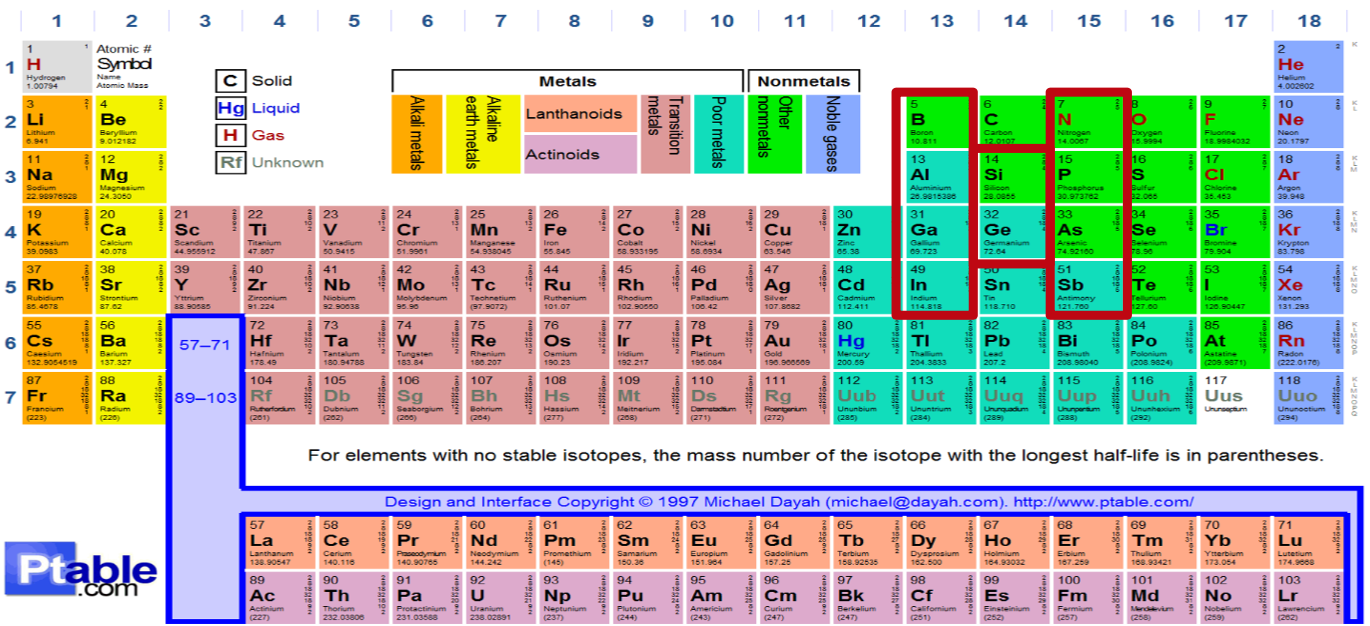
\includegraphics[scale=0.4,angle=0]{tavola_periodica.png}
\caption{Tavola periodica}
\end{figure}

I più comuni semiconduttori sono il \textbf{silicio} e il \textbf{germanio} che, trovandosi nella $IV^{a}$ colonna della tavola periodica, hanno quattro elettroni nell'orbitale più esterno. Sono gli unici semiconduttori \textbf{non composti}, cioè costituiti da atomi di un solo tipo. Altri possibili semiconduttori sono i seguenti composti \textbf{binari}: arseniuro di gallio GaAs, nitruro di gallio GaN, fosfuro di indio InP e il carburo di silicio SiC (un composto 4\,-\,4 perché sia il carbonio che il silicio appartengono alla quarta colonna), tutti formati da un elemento della $III^{a}$ colonna e da uno della $V^{a}$ e per questo si comportano come un elemento della quarta colonna (perché in media hanno quattro elettroni).\\Dunque, nei semiconduttori gli atomi coinvolti sono tutti collocati a cavallo della $IV^{a}$ colonna della tavola periodica: quella del carbonio (ma da solo non è usato come semiconduttore), silicio e germanio che hanno orbitali mezzi pieni e mezzi vuoti; cioè ci sono quattro elettroni e quattro spazi vuoti.

Di base, un materiale semiconduttore da solo è un materiale debolmente o per niente conduttore e non esprime, da solo, nessuna particolare proprietà, tuttavia diventa un materiale utilizzabile nel campo dell'elettronica quando viene \textbf{drogato}. Durante questo processo si parte da una matrice cristallina di materiale base che deve essere un materiale della quarta colonna, per esempio il silicio, e per \textbf{diffusione} si inserisce al suo interno una piccola quantità (circa una parte per miliardo) di \textbf{impurità}, ovvero di materiali appartenenti alla $III^{a}$ o alla $V^{a}$ colonna; generalmente sono rispettivamente il boro \textbf{B} e il fosforo \textbf{P}.

Nel caso del fosforo si parla di \textbf{impurità di quinta colonna} caratterizzata dall'avere un \textit{eccesso} di elettroni perché il fosforo ne ha cinque rispetto ai quattro del silicio. Il fosforo, inserito nella matrice di silicio, fornisce degli elettroni aggiuntivi (rappresentati tramite una carica negativa) rispetto al \textit{reticolo di base}, la struttura della matrice rimane la stessa, ovvero il reticolo del silicio, ma di tanto in tanto ci sono degli elettroni in più che rendono il materiale più \textbf{elettronegativo}, cioè più disponibile a fornire degli elettroni, e quindi si guadagna una certa conducibilità elettrica. In generale, quando si aggiunge un materiale \textit{drogante} di quinta colonna, il materiale che si ottiene è detto di \textbf{tipo n}. Quindi se il materiale di base è drogato da una impurità di tipo n significa che c'è un eccesso di elettroni, cioè di cariche negativa all'interno del materiale.

Nel caso del boro, o più in generale di un drogante di terza colonna, si parla di \textbf{impurità di terza colonna} caratterizzata dall'avere un \textit{difetto} di elettroni perché l'elemento di terza colonna ha solo tre elettroni rispetto ai quattro del reticolo. A livello pratico è come se per ogni impurità nella matrice si avesse un piccolo buco, cioè una mancanza di elettrone che prende il nome di \textbf{lacuna} e in genere si modella come se fosse una \textit{carica positiva}, infatti matematicamente le lacune vengono trattate come se fossero delle vere cariche positive per far tornare correttamente i conti. Il materiale ottenuto tramite questo secondo tipo di impurità è detto di \textbf{tipo p}.

Nell'interazione tra un materiale di tipo p e un materiale di tipo n si nota che gli elettroni in eccesso nel materiale di tipo n passano attraverso le lacune del materiale di tipo p.

Il drogaggio in entrambi i casi può essere fatto sia utilizzando un materiale \textbf{puro} come il silicio e il germanio, oppure tramite un materiale \textbf{composto}, l'importante è che il materiale sia mediamente di quarta colonna. Il silicio è di gran lunga il materiale più usato però non è strettamente quello che ma prestazioni migliori, il germanio viene maggiormente utilizzato per i dispositivi a radiofrequenza ma è molto più raro come lo sono anche GaAs, GaN e InP. SiC è costituito da carbonio e silicio che sono facilmente reperibili ma deve essere costruito quindi rimane comunque mediamente costoso.\\Lo specifico materiale da utilizzare dipende dall'elettronica che si deve andare a costruire. Per l'elettronica digitale, come celle logiche e microprocessori, si può utilizzare la tecnologia del silicio più i vari droganti. Per l'elettronica di potenza ad alte prestazioni si tende a preferire il nitruro di gallio o il carburo di silicio per le loro caratteristiche. Per i dispositivi optoelettronici, per esempio i LED, si usano invece il fosfuro di indio e l'arseniuro di gallio.

\section{Giunzioni PN}
Si ottengono quando si fa un drogaggio del silicio, cioè quando si aggiunge un materiale al silicio puro. L'aspetto particolare non è tanto il drogaggio del materiale di base quanto il mettere in contatto materiali drogati di tipo diverso, p ed n.

Nel caso dei materiali di tipo p si va a studiare il numero di \textbf{accettori}, indicato con $N_{a}$, rappresentante il numero di \textit{lacune} per unità di volume. Al contrario, per i materiali di tipo n si va a studiare il numero $N_{d}$ rappresentante il numero di \textbf{donatori} per unità di volume, cioè il numero di atomi che donano un elettrone. Sia $N_{a}$ che $N_{d}$ sono dell'ordine di $10^{-9}\,, 10^{-10}$ cioè un atomo ogni $10^{10}$ circa è un drogante di tipo p o n.

Più il silicio di base viene drogato e più esso tenderà a diventare un materiale con un comportamento sempre più lontano da quello del silicio di base. Di base il silicio si organizza in una \textit{matrice cristallina}, cioè come un \textit{cristallo} che non lascia passare lacune ed elettroni ma aggiungendo delle impurità si rendendo disponibili elettroni in più oppure delle lacune in cui potranno finire degli elettroni.

Per ottenere le \textbf{giunzioni p\,-\,n} si parte da una matrice di silicio la quale, tramite un processo di diffusione dall'alto, viene prima drogata con un drogante di tipo n andando a creare una \textit{tasca} e poi su una certa sezione già drogata della tasca viene ulteriormente inserito un drogante di tipo p (la diffusione può essere effettuata selettivamente in specifiche aree della matrice in base alle esigenze). La giunzione pn si formerà quindi lungo il \textit{bordo di confine} tra il drogaggio di tipo p e quello di tipo n.
\begin{figure}[ht]
\centering
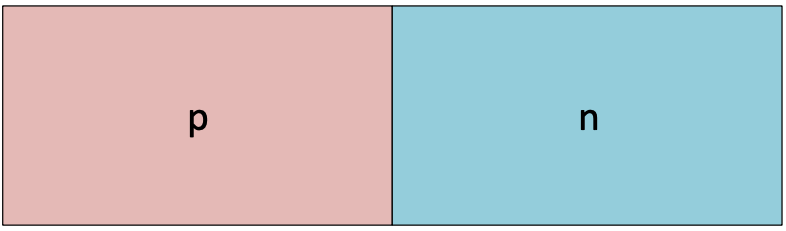
\includegraphics[scale=0.4,angle=0]{giunzione_pn.png}
\caption{Giunzione PN}
\end{figure}

Preso un materiale di tipo p avente un eccesso di lacune rispetto al reticolo e uno di tipo n con un eccesso di elettroni, nonostante le impurità i due materiali sono entrambi \textit{elettricamente neutri}. Lo sbilanciamento di elettroni in un lato e di lacune disponibili nell'altro fa sì che nel momento in cui un materiale di tipo p e uno di tipo n entrano in contatto si verifica un fenomeno di \textbf{migrazione} per cui statisticamente gli elettroni in eccesso nel materiale di tipo n tendono a migrare nel materiale di tipo p avente dello spazio libero dato dalle lacune.
\begin{figure}[h]
\centering
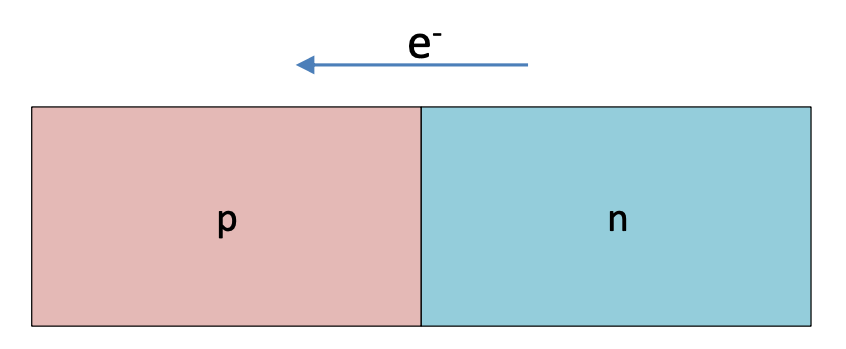
\includegraphics[scale=0.4,angle=0]{giunzione_pn_elettroni.png}
\caption{Migrazione degli elettroni}
\end{figure}

Via via che gli elettroni passano nel materiale di tipo p ognuno di essi si inserisce in una lacuna, riempiendola. Nel far ciò il materiale di tipo p passa dall'essere un materiale neutro (era un materiale della terza colonna con tre protoni e tre elettroni) ad essere \textit{negativamente carico} e questo comporta che la carica negativa che si è venuta a creare emette un \textbf{campo elettrico} che respinge altre cariche negative. Per cui, via via che gli elettroni passano nel materiale di tipo p tale materiale diventa più carico negativamente e si genera un campo elettrico negativo, inoltre gli elettroni che sono passati hanno liberato posti all'interno del materiale di tipo n nel quale quindi si crea una \textit{carica positiva}. Si arriva quindi ad un punto in cui sono passati un certo numero di elettroni che hanno generato un campo elettrico che impedisce ad altri elettroni nel materiale di tipo n di passare, si ha un \textbf{equilibrio}.

All'equilibrio, un certo numero di elettroni è passato nel materiale di tipo p e ha creato una zona a carica nettamente negativa e si sono formate un certo numero di lacune nel materiale di tipo n che hanno creato una zona a carica nettamente positiva. In queste condizioni, non è possibile far fluire ulteriori elettroni perché verrebbero respinti dal campo elettrico generato dagli elettroni passati in precedenza.
\begin{figure}[ht]
\centering
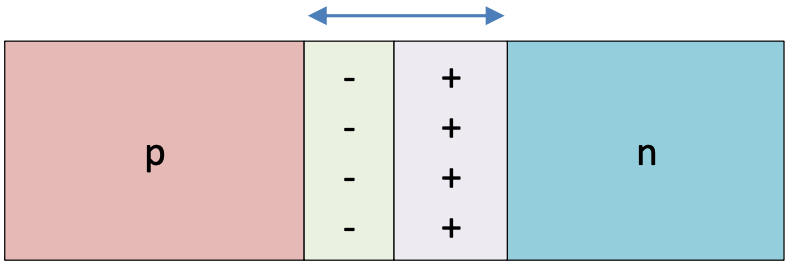
\includegraphics[scale=0.4,angle=0]{giunzione_pn_equilibrio.png}
\caption{Giunzione PN all'equilibrio}
\end{figure}

Nella zona a carica negativa non c'è più spazio per poter far arrivare e ospitare ulteriori elettroni e, analogamente, nella zona a carica positiva sono presenti tutti quegli atomi che in precedenza avevano cinque elettroni e ora ne hanno quattro, quindi non si possono più spostare altri elettroni perché si è tornati alla conformazione del reticolo cristallino del silicio con quattro elettroni; è silicio carico positivamente ma non ha elettroni trasferibili. Questo sbilanciamento di carica (da un lato una carica negativa netta e dall'altro una carica positiva netta) come già detto provoca un campo elettrico che blocca l'ulteriore diffusione di elettroni e la regione in cui sono presenti le due cariche nette opposte è chiamata \textbf{regione di svuotamento} o \textbf{regione di carica spaziale}. Di svuotamento nel senso che in quella regione sono stati eliminati tutti i \textit{portatori} di carica; di carica spaziale nel senso che questo procedimento ha portato a creare una \textit{densità di carica} positiva e negativa che implica la formazione di un campo elettrico.
\begin{figure}[h]
\centering
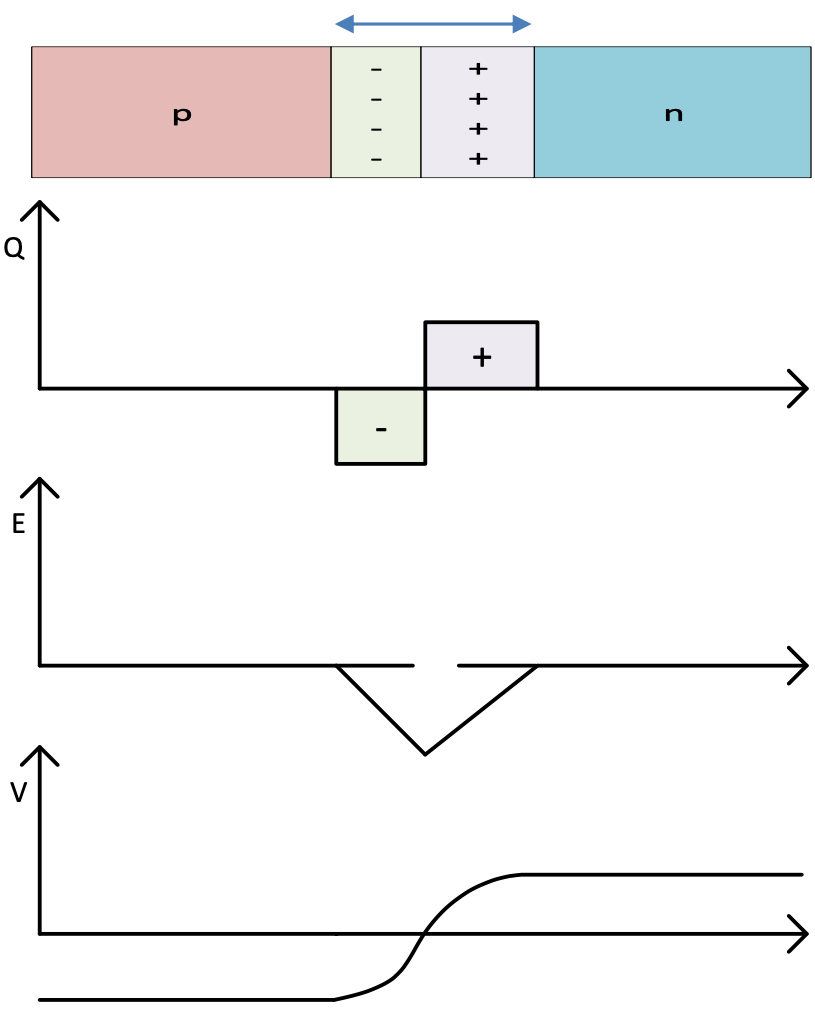
\includegraphics[scale=0.4,angle=0]{giunzione_pn_grafici.png}
\caption{Cariche, campo elettrico e potenziale della giunzione PN}
\label{grafici}
\end{figure}

Come si nota in figura \ref{grafici}, nel dominio della carica nella ragione di svuotamento relativa alla zona p si crea una regione di cariche nettamente negative mentre in quella relativa alla zona n se ne crea una di cariche nettamente positiva.

Dallo studio della carica è possibile ricavare informazioni relative sia al campo elettrico che al potenziale. Percorrendo l'asse \textit{x} da sinistra verso destra e integrando rispetto alle cariche incontrate, cioè integrando la \textit{distribuzione} di carica (la funzione rappresentata nel primo grafico - per semplicità si è presa esattamente rettangolare cioè una distribuzione uniforme), si ricava il campo elettrico $E(x) = \int q\,dx$ (secondo grafico di figura \ref{grafici}) che è una funzione decrescente nell'intervallo in cui ci sono solo cariche negative, ha il minimo in corrispondenza della giunzione pn e da lì diventa una funzione crescente dal momento in cui si entra nella zona con carica positiva netta. Sia la crescita che la decrescita sono entrambe \textit{lineari} avendo supposto una distribuzione uniforme in entrambe le zone. Inoltre la funzione $E(x)$ nei due estremi vale $0$ perché la quantità di carica positiva e negativa è \textit{la stessa} e questo è dovuto al fatto che ad ogni elettrone passato corrisponde una lacuna lasciata.

L'\textit{estensione} della zona a carica positiva e di quella a carica negativa non sono uguali perché l'estensione fisica della regione di svuotamento sia nel lato p che nel lato n è \textit{direttamente proporzionale} a quante lacune e a quanti elettroni ci sono per unità di volume. Si scambia la stessa quantità di elettroni e lacune ma la dimensione delle due zone dipende dalla quantità di portatori, cioè dipende dalla \textit{densità} del drogante. Se per esempio si suppone che il drogaggio della parte p sia il doppio di quello della parte n (quindi $N_{a} > N_{d}$), siccome il numero totale di elettroni è lo stesso a destra e a sinistra, una volta riempita tutta la regione di svuotamento si sa che ci sono $N_{a}$ elettroni per unità di volume nella zona costituente la carica negativa netta. Posta $x_p$ la lunghezza della zona a carica negativa netta e $x_{n}$ quella della zona a carica positiva netta, $N_{a} \cdot x_{p}$ rappresenta la quantità di elettroni nella zona p e deve essere uguale alla quantità di cariche positive nella zona n, cioè deve valere:
\begin{equation}
    N_{a} \cdot x_p = N_{d} \cdot x_n
    \label{giunzione_pn}
\end{equation}
che riassume il fatto che un elettrone che si sposta dalla zona n alla zona p lascia una carica positiva nella zona n e porta una carica negativa nella zona p e gli spazi utilizzabili sono quelli dovuti alle lacune e alle cariche negative che sono state create con il drogaggio. In base alla \eqref{giunzione_pn} l'estensione della regione di svuotamento è \textit{inversamente proporzionale} alla quantità di drogante: più la regione è drogata e più sarà sottile e viceversa. Questo significa ancora che nel primo grafico di figura \ref{grafici} i due rettangoli, aventi base $x_{p}$ e $x_{n}$ e altezza rispettivamente $N_{a}$ e $N_{d}$, devono avere la stessa area.

Integrando il campo elettrico $E(x)$ si ottiene il \textbf{potenziale} che, a meno di una costante presa negativa, parte negativo e diventa positivo, cioè nella zona n è più positivo che nella zona p (terzo grafico di figura \ref{grafici}).

\section{Diodi}
Il risultato finale di quanto detto è la creazione di un campo elettrico e di una differenza di potenziale, cioè una \textbf{tensione}, tra la zona n e la zona p. La differenza di potenziale fa sì che gli ulteriori elettroni che si trovano nella zona n (quindi non quelli che vanno a formare la carica positiva netta) siano bloccati e non possano passare nella zona p. Analogamente, anche le lacune non possono andare dalla zona p a quella n perché trovano un potenziale positivo e vengono quindi respinte. Ci si trova in una condizione di equilibrio. Il dispositivo così ottenuto è chiamato \textbf{diodo}; in particolare è un \textit{diodo a giunzione pn}.
\begin{figure}[h]
\centering
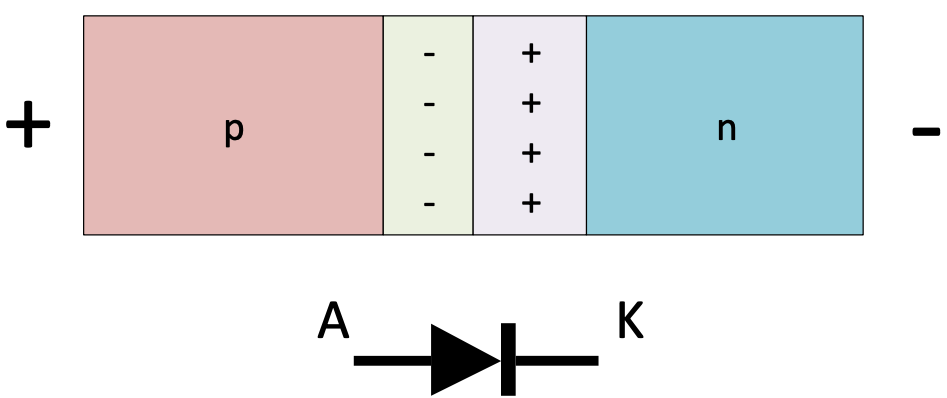
\includegraphics[scale=0.4,angle=0]{diodo.png}
\caption{Struttura e simbolo di un diodo in \textit{polarizzazione diretta}}
\end{figure}

Il diodo è formato da due terminali chiamati \textbf{anodo} e \textbf{catodo}, indicati con \textit{A} e \textit{K} e corrispondenti rispettivamente alla zona \textit{p} contente le lacune e alla zona \textit{n} contente gli elettroni. La freccia che compare nel simbolo del diodo indica il verso in cui scorre la \textit{corrente} (intesa come cariche positive): essa scorre dall'anodo verso il catodo. Se la corrente si muove dall'anodo verso il catodo significa che gli elettroni si spostano nel verso opposto: dal catodo all'anodo.

Come detto in precedenza, la barriera di potenziale che si viene a creare in corrispondenza delle due cariche nette e della giunzione impedisce agli elettroni di spostarsi dalla zona n alla zona p cioè dal catodo all'anodo. Tuttavia questo risulta essere vero fintanto che non si applica esternamente un certo \textit{potenziale}. In particolare, se si applica un potenziale \textit{positivo} all'anodo e \textit{negativo} al catodo ci si trova nelle condizioni di \textbf{polarizzazione diretta} tramite la quale il potenziale positivo applicato all'anodo fa alzare il potenziale della regione p e il potenziale negativo applicato al catodo fa abbassare il potenziale della regione n. Inoltre, fintanto che non c'è corrente all'interno della zona p non c'è caduta di potenziale, quindi il potenziale all'estrema sinistra è lo stesso potenziale del punto in cui inizia l'area con la carica negativa netta, lo stesso vale per la zona n. Con l'applicazione di potenziale esterno ai due estremi la curva tende a diventare sempre più piatta tendendo a diventare parallela all'asse \textit{x}; in queste condizioni gli elettroni e le lacune non incontrano più nessuna barriera di potenziale, quindi nessun ostacolo, e per questo sono liberi di fluire. Via via che si incrementa il potenziale in p e lo si abbassa in n, un po' di elettroni dal generatore esterno passano attraverso la zona n e vanno a neutralizzare la carica positiva netta. A questo punto, per effetto del \textit{bilanciamento} delle cariche, per ogni carica positiva che viene bilanciata a destra, un elettrone nella carica negativa netta si stacca e va verso il generatore passando attraverso la zona p e infine uscendo dal diodo Più questo processo va avanti e poi la regione di svuotamento diventa più stretta fino a svanire del tutto, una volta eliminata gli elettroni sono liberi di fluire.

Una volta raggiunta una certa tensione viene quindi annullata la barriera di potenziale e gli elettroni sono liberi di scorrere nel materiale pn. Dunque, applicando una tensione maggiore di una certa soglia inizia a scorrere corrente. Questa tensione soglia prende il nome di \textbf{tensione del diodo} (del potenziale interno che si era creato intorno alla giunzione pn con le due cariche nette opposte), viene indicata con $V_{D}$. Per un diodo al \textit{silicio} $V_D \approx 0,7\,V$, il che significa che se col generatore si supera la tensione di $0,7\,V$ si riesce ad annullare la barriera di potenziale nel mezzo del diodo pn e inizia a scorrere corrente con un andamento \textbf{esponenziale} con la tensione applicata al diodo:
\begin{equation}
    I_{D} = I_{0}\,(e^{(V_{D}/nV_{T})} - 1)
    \label{corrente_id}
\end{equation}
Per cui, fino a $0,7\,V$ non succede niente, superata tale soglia la corrente inizia a crescere esponenzialmente perché non incontra più nessun ostacolo.

Inizialmente si era detto che se non scorre corrente la parte di materiale p ed n non producono una caduta di tensione, però in realtà intrinsecamente le due parti di materiale p ed n sono anche \textit{conduttori} quindi presentano una loro certa \textbf{resistività}. Dunque se si volesse fare una rappresentazione veritiera del circuito, oltre al generatore e al diodo \textit{ideale} bisognerebbe aggiungere due \textbf{resistenze}: una lato anodo rappresentante la conducibilità del materiale p e una lato catodo rappresentante quella del materiale n. Da questa rappresentazione si può quindi vedere come nella realtà ai capi della giunzione arrivi meno tensione di quella effettiva. 

Sapendo che la tensione delle resistenze è data da $V = R \cdot I$, la curva è esponenziale un volta superata la soglia di $0,7\,V$ ma ad un certo punto la tensione che si genera per \textit{caduta resistiva} è così grande che la tensione ai capi del diodo non cresce più, a quel punto la corrente $I_{D}$ non sarà più esponenziale ma \textit{lineare}. Meno corrente il diodo è in grado di portare e tanto prima di entrerà nella regione a crescita lineare.

Nella norma la regione di tipo p e quella di tipo n non sono drogate in maniera omologa ma una delle due è molto più drogata dell'altra. Il più delle volte è la regione n ad essere più drogata della regione p, cioè vale che $N_{d} >> N_{a}$. In queste condizioni ci sono tanti portatori di tipo n nella zona n (inteso come densità) ma ci sono poche lacune nella zona p, quindi quando un elettrone passa nella zona p si trova in una sorta di mare deserto di lacune. Per questa situazione si parla di \textbf{portatori minoritari} intendo il fatto che i portatori, cioè le lacune, sono molto sparsi e questo comporta che si hanno fenomeni di diffusione degli elettroni nel lato p e sono fenomeni non simmetrici, cioè non si osservazione la stessa situazione anche per la lacune nel lato n. L'aspetto principale è che via via che nel diodo sono presenti elettroni, questi si vanno ad accumulare nella parte di tipo p causando un fenomeno detto di \textbf{accumulo di carica} che, si vedrà più avanti, ha un effetto indesiderato.
\\\\Le considerazioni fatte finora sono relative al caso di polarizzazione diretta in cui si applica un potenziale positivo all'anodo e uno negativo al catodo. Nel caso contrario, detto \textbf{polarizzazione inversa} in cui si applica un potenziale negativo all'anodo e uno positivo al catodo, riprendendo l'andamento del potenziale in figura \ref{grafici}, il potenziale negativo applicato all'anodo fa abbassare ulteriormente il potenziale della regione p e il potenziale positivo applicato al catodo fa alzare ancora di più il potenziale della regione n.
\begin{figure}[h]
\centering
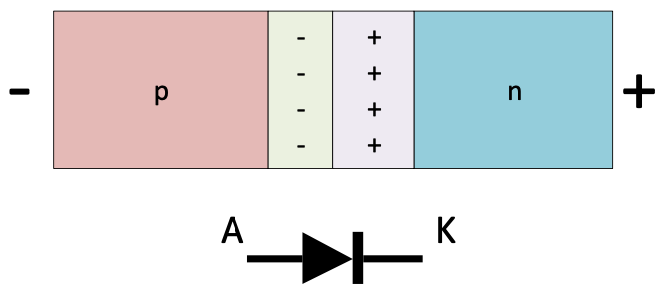
\includegraphics[scale=0.4,angle=0]{diodo_polarizzazione_inversa.png}
\caption{Diodo in \textit{polarizzazione inversa}}
\end{figure}
\\Questo comporta un aumento del valore assoluto della barriera di potenziale che diventerà più ripida. Inoltre, gli elettroni immessi nella zona p tramite il generatore esterno, si vanno ad aggiungere alla regione di svuotamento originale e, viceversa, nella zona n degli elettroni abbandonano la zona uscendo dal diodo. Il risultato netto è che la regione di svuotamento si \textit{allarga} con un corrispondente incremento della barriera di potenziale: i due rettangoli nel primo grafico di figura \ref{grafici} diventano più grandi, quindi aumenta anche il campo elettrico $E(x)$. Più aumenta la barriera di potenziale, più si accumulano cariche e più diventa difficile lo scorrimento della corrente attraverso il diodo. In realtà si ha comunque una corrente che scorre dal catodo all'anodo ed è definita dalla formula \eqref{corrente_id} che quindi vale sia per la polarizzazioni diretta che per quella inversa. In particolare, la corrente che scorre in polarizzazione inversa (anche detto \textbf{reverse bias}) è $I_{0}$ che è molto bassa (dell'ordine di $10^{-7} A$) ma comunque non nulla. Questa \textit{corrente di perdita} sarà tanto più piccola tanto più si sarà fatta attenzione nel progettare il diodo in modo tale che non ci sia e, generalmente, è proporzionale a quanta corrente può scorrere nel diodo nel caso di polarizzazione diretta o \textbf{forward bias}: diodi più grandi avranno corrente di perdita più grande e viceversa.

Il campo elettrico, come si vede nel secondo grafico di figura \ref{grafici}, ha il valore massimo in corrispondenza del confine tra la giunzione p e la giunzione n. In questo momento la parte centrale del diodo si comporta come un materiale \textbf{dielettrico} perché non conduce corrente a causa del fatto che le cariche sono tutte bloccate nella regione di svuotamento. Ma un materiale dielettrico non conduce corrente fino a quando non si supera la sua \textbf{rigidità dielettrica}. Il silicio ha un limite di rigidità dielettrica oltre la quale il materiale si \textit{rompe} (si dice che va in \textbf{breakdown}): il campo elettrico è così forte che le cariche elettriche da una parte vengono tirate dalla parte opposta fino ad essere \textit{strappate} dal reticolo cristallino e, a quel punto, inizia a scorrere corrente. Quindi il diodo, che in polarizzazione inversa non fa quasi scorrere corrente, una volta superata una certa soglia di rigidità dielettrica, detta \textbf{tensione di breakdown}, va in breakdown e da quel momento inizia a scorrere una corrente che cresce in maniera illimitata e improvvisa.
\begin{figure}[h]
\centering
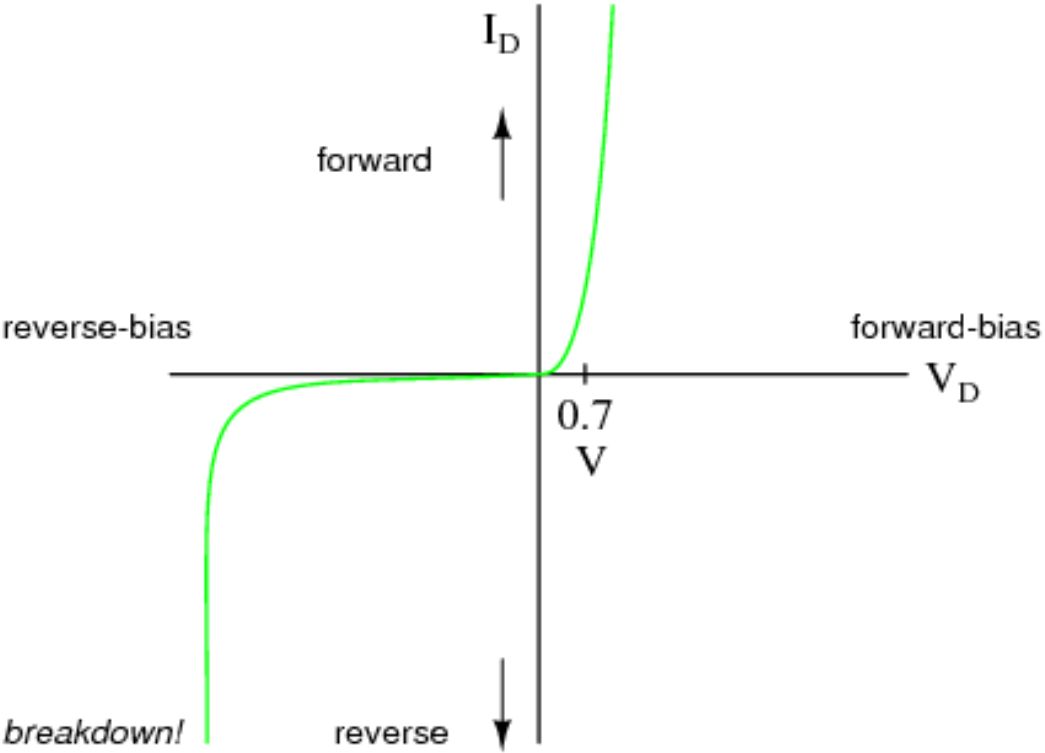
\includegraphics[scale=0.4,angle=0]{corrente_id.png}
\caption{Andamento della corrente nel diodo in polarizzazione diretta e inversa}
\end{figure}

In base a come sono costruiti diodo e circuito, il breakdown può essere \textit{reversibile}. Se all'interno del circuito (considerando un generatore ideale) la corrente non viene limitata in qualche modo (per esempio tramite delle resistenze) il diodo non è recuperabile dopo il breakdown. Ci sono due categorie di diodi: i diodi costruiti per andare in breakdown e quelli costruiti per non andarci; questi ultimi è molto probabile che effettivamente si rompano se vanno in breakdown indipendentemente dalla corrente. I diodi che invece sono costruiti appositamente per andare in breakdown sono chiamati \textbf{diodi Zener} e non si danneggiano andando in breakdown ma bisogna comunque limitare la corrente per esempio con una resistenza in serie per avere un corrente quasi lineare e quindi facilmente controllabile.
\begin{figure}[h]
\centering
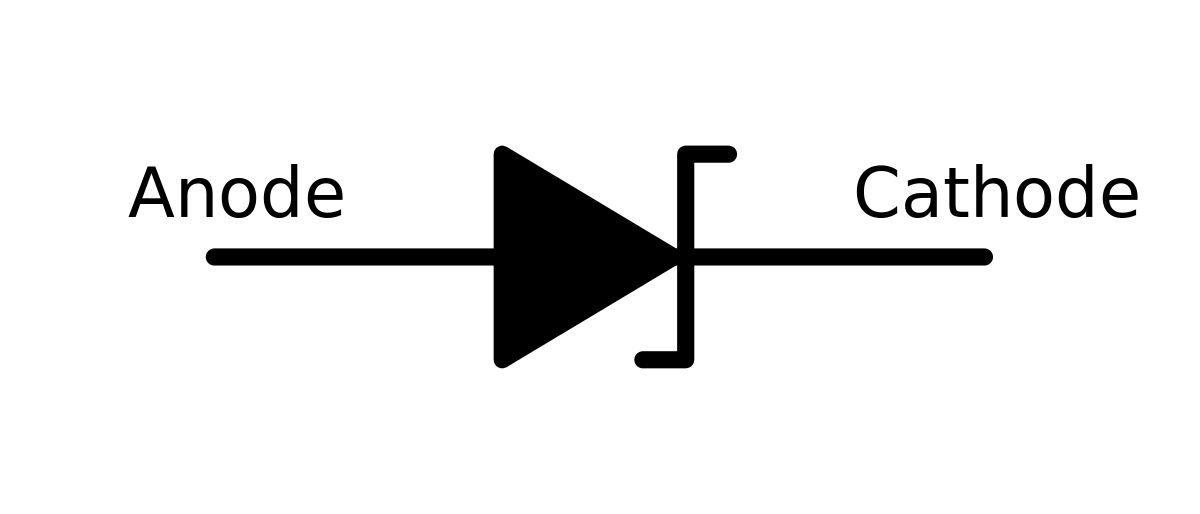
\includegraphics[scale=0.15,angle=0]{diodo_zener.png}
\caption{Simbolo del diodo Zener}
\end{figure}
\\In passato venivano usati per controllare la tensione ed è l'unico diodo che sopporta il breakdown inverso ma bisogna inserire una \textit{resistenza di limitazione}.
\\\\Nel contesto dell'elettronica digitale, in logica binaria, per una tensione $V_{D}$ compresa tra $0\,V$ e $0,7\,V$ si considera una corrente di $0\,A$ mentre oltre gli $0,7\,V$ si considera una corrente di $1\,A$, cioè infinita. Per tensioni negative, per $V_{D}$ compresa tra $0\,V$ e la tensione di breakdown si considera una corrente di $0\,A$ e oltre la tensione di breakdown si considera corrente infinitamente negativa. Nella realtà però il diodo è un dispositivo analogico caratterizzato da non avere cambi repentini di intensità di corrente.

\section{Diodi speciali}
Oltre al diodo Zener e ai diodi pn al silicio che si usano per controllare il verso di scorrimento della corrente, ci sono altre tipologie di diodi costruibili sfruttando ancora le proprietà dei materiali semiconduttori.
\begin{enumerate}
    \item \textbf{Fotodiodo}: è un dispositivo optoelettronico, cioè un dispositivo che sfrutta il dualismo tra energia e lunghezza d'onda (cioè tra fotone e l'energia che esso porta) per far sì che nel dispositivo a semiconduttore la luce che incide sul dispositivo stesso possa produrre degli effetti. A differenza di altri dispositivi optoelettronici che sono neri per non modificare il loro funzionamento a causa della luce, il fotodiodo è \textit{trasparente}. Il principio di funzionamento è del tutto analogo a quello della cella fotovoltaica: viene emessa corrente quando della luce incide sul fotodiodo. Per usarlo lo si polarizza in inversa e se della luce lo colpisce, se il fotone colpisce la regione di svuotamento, l'energia associata al fotone $e = \hbar \cdot \nu$ (con $\nu$ l'inverso della lunghezza d'onda) è in grado di prendere un elettrone nel reticolo cristallino e portarlo dalla \textbf{banda di valenza} nella \textbf{banda di conduzione} così che l'elettrone si stacca dalla sua lacuna, si crea una coppia elettone-lacuna liberi che è in grado di seguire il campo elettrico che si è creato tramite il quale la corrente scorre verso l'anodo, e si ha un passaggio di corrente. Quindi il diodo, che di base in polarizzazione inversa non conduce corrente, quando viene illuminato da una luce che abbia sufficiente energia per poter far passare gli elettroni dalla banda di valenza a quella di conduzione riesce a condurre corrente anche in condizioni di polarizzazione inversa. Si può usare per rilevare una radiazione luminosa incidente (per esempio in un telecomando a raggi infrarossi) oppure nei pannelli fotovoltaici in cui il pannello non è altro che un grande diodo pn al silicio e quando su di esso incide della luce solare diventa lui stesso un generatore di corrente con la corrente positiva uscente dall'anodo e la tensione che si genera ai capi del diodo che è sicuramente \textit{minore o uguale} della tensione di soglia del diodo stesso. Se la tensione che si genera fosse maggiore di $0,7\,V$ il diodo si polarizzerebbe direttamente e al suo interno vorrebbe scorrere una corrente contraria, dall'anodo al catodo. Normalmente una diodo al silicio per applicazioni fotovoltaiche genera tra gli $0,5$ e gli $0,6$ volt.
    \item \textbf{LED}: anche questo è un dispositivo optoelettronico che sostanzialmente ha un funzionamento opposto a quello del fotodiodo. È un dispositivo costruito in modo tale che quando viene polarizzato direttamente sia facile che nella regione di svuotamento si vadano a ricombinare elettroni e lacune; cioè è costruito in modo tale che gli elettroni che sono in banda di conduzione possano cadere in banda di valenza, così da poter liberare un fotone. La lunghezza d'onda del fotone liberato è \textit{inversamente proporzionale} all'energia (quindi la frequenza della radiazione luminosa emessa è direttamente proporzionale all'energia), quindi ad un salto energetico molto alto (barriera di potenziale alta) corrisponderà una lunghezza d'onda molto bassa cioè l'emissione del diodo si sposta verso gli ultravioletti; al contrario, se la barriera di potenziale è bassa l'emissione si sposta verso gli infrarossi. Accanto agli infrarossi c'è il \textit{rosso}, accanto agli ultravioletti c'è il \textit{viola}, nel mezzo partendo dal viola ci sono il blu, il verde, il giallo, l'arancione e infine il rosso. Dunque la lunghezza d'onda della luce emessa dal LED è esattamente determinata dalla sua distanza tra la banda di valenza e quella di conduzione, e a sua volta quella distanza è proporzionata dalla tensione che cade sul diodo, per questo il diodo LED è un diodo che normalmente ha una tensione di soglia \textit{molto alta}, soprattutto nel visibile e nell'ultravioletto. Inoltre, la tensione che cade ai capi del diodo, proprio perché è fatto per avere una barriera di potenziale grande, è tendenzialmente $> 1,5\,V$: per i LED \textit{rossi} è tipicamente $1,5\,V$, per i \textit{verdi} circa $1,8\,V$, per quelli \textit{blu} circa $2,2\,V$, per i diodi \textit{ultravioletti} è intorno ai $3\,V$, per i diodi \textit{infrarossi}, in particolare quelli nel vicino infrarosso, è circa $1,2\,V$. In ogni caso, la caduta di potenziale è proporzionata all'energia dell'emissione luminosa e tanto più l'emissione luminosa si sposta verso gli ultravioletti, tanto più è energetica e quindi tanto maggiore è la caduta di potenziale ai capi del diodo.
    \item \textbf{Diodo Shottky}: diodo particolare in cui la giunzione pn è fatta da un \textit{metallo} (per esempio l'\textit{alluminio} che è un materiale di $III^{a}$ colonna) nella zona p e da un \textit{semiconduttore} nella zona n. Questo accoppiamento fa sì che la regione di svuotamento si estenda solo nel lato del semiconduttore, nel metallo non esiste la regione di svuotamento perché la strutta molecolare di un metallo è il \textbf{mare di elettroni} in cui gli elettroni sono sempre liberi di muoversi: non si crea la regione di svuotamento ma il campo elettrico si. Questa caratteristica permette di avere una tensione di soglia \textit{minore} di quella di un diodo al silicio perché di fatto la regione di svuotamento è la metà di quella che si avrebbe normalmente. Come detto in precedenza, mentre scorre corrente in un diodo normale si accumulano cariche minoritarie nella parte p. Questo comporta che quando si vuole spegnere il diodo, quindi $V_{D}$ diventa negativa perché si fa una polarizzazione inversa, esso si spegne lentamente, cioè $I_{D}$ scende lentamente ala valore previsto nel caso statico (invece si accende facilmente non appena viene polarizzato) perché ha accumulato cariche nella parte p che lo tengono ancora acceso. La corrente $I_{D}$ passa dall'essere positiva all'essere negativa per un certo tempo, fintanto che gli elettroni accumulati non vengono liberati. Indipendentemente dalla polarizzazione, passa comunque corrente. Tutto questo non succede nel diodo Shottky in cui, poiché la carica netta nella parte p non esiste, non esiste un accumulo di cariche bloccate nelle lacune e questo fa sì che quando il diodo passa in polarizzazione inversa, si spegne immediatamente cioè si comporta dinamicamente come un diodo ideale.
\end{enumerate}

\chapter{BJT}
\chapter{MOS}
\chapter{RTL e TTL}
\chapter{Logica sequenziale e Flip-Flop}
\chapter{Circuiti integrati commerciali}
\chapter{Convertitori DA e AD}
\chapter{Microcontrollori}
\end{document}
